\documentclass[../report.tex]{subfiles}
\begin{document}
    
    \begin{frame}
        \frametitle{4a: PF Occlusions}
        \begin{figure}[!htb]
            \centering
            \frame{
\includegraphics[keepaspectratio,height=0.65\textheight,width=0.45\textwidth]{ps5-4-a-1}}
            \caption{ps5-4-a-1}
        \end{figure}
    \end{frame}

    \begin{frame}
        \frametitle{4a: PF Occlusions (cont.)}
        \begin{figure}[!htb]
            \centering
            \frame{
\includegraphics[keepaspectratio,height=0.65\textheight,width=0.45\textwidth]{ps5-4-a-2}}
            \caption{ps5-4-a-2}
        \end{figure}
    \end{frame}

    \begin{frame}
        \frametitle{4a: PF Occlusions (cont.)}
        \begin{figure}[!htb]
            \centering
            \frame{
\includegraphics[keepaspectratio,height=0.65\textheight,width=0.45\textwidth]{ps5-4-a-3}}
            \caption{ps5-4-a-3}
        \end{figure}
    \end{frame}

    \begin{frame}
        \frametitle{4a: PF Occlusions (cont.)}
        \begin{figure}[!htb]
            \centering
            \frame{
\includegraphics[keepaspectratio,height=0.65\textheight,width=0.45\textwidth]{ps5-4-a-4}}
            \caption{ps5-4-a-4}
        \end{figure}
    \end{frame}

    \begin{frame}[t]
        \frametitle{4: Text response}
        \begin{normalsize}
            \begin{itemize}
                \setlength\itemsep{1em}\fontsize{6pt}{6pt}

                \item[]{\textbf{\selectfont\textcolor{blue}{ Describe what you did. How did you modify the Particle Filter class to continue tracking after occlusions? }}}
                
                \item[]\textbf{\documentclass[../report.tex]{subfiles}
\begin{document}
    
    \begin{frame}
        \frametitle{4b: Viola Jones Features}
        \begin{figure}[!htb]
            \centering
            \frame{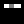
\includegraphics[keepaspectratio,height=0.65\textheight,width=0.45\textwidth]{ps6-4-b-1}}
            \caption{ps6-4-b-1}
        \end{figure}
    \end{frame}

    \begin{frame}
        \frametitle{4b: Viola Jones Features}
        \begin{figure}[!htb]
            \centering
            \frame{
\includegraphics[keepaspectratio,height=0.65\textheight,width=0.45\textwidth]{ps6-4-b-2}}
            \caption{ps6-4-b-2}
        \end{figure}
    \end{frame}

    \begin{frame}[t]
        \frametitle{4b: Analysis}
        \begin{normalsize}
            \begin{itemize}
                \setlength\itemsep{1em}\fontsize{6pt}{6pt}

                \item[]{\textbf{\selectfont\textcolor{blue}{ Report the classifier accuracy both the training and test sets with a number of classifiers set to 5. What do the selected Haar features mean? How do they contribute in identifying faces in an image? }}}
                
                \item[]\textbf{% A line starting with a % character is a comment and wont be included in the report.
% Always use two backslashes like \\ to insert a new line. Take a look at the example below.
I think \\
my answer is ...
}
            \end{itemize}
        \end{normalsize}
    \end{frame}

    \begin{frame}
        \frametitle{4c: Viola Jones Face Recognition}
        \begin{figure}[!htb]
            \centering
            \frame{
\includegraphics[keepaspectratio,height=0.65\textheight,width=0.45\textwidth]{ps6-4-c-1}}
            \caption{ps6-4-c-1}
        \end{figure}
    \end{frame}
    
\end{document}}
            \end{itemize}
        \end{normalsize}
    \end{frame}

    
\end{document}